% ============================================================
%  IEEE Transactions — Kill-Chain MaxSAT Honeypot Placement
%  v8 — Real Experimental Figures + Updated XLarge Numbers
%       + Mininet Emulation + All Existing Boxes Retained
% ============================================================
\documentclass[journal]{IEEEtran}

\usepackage{amsmath,amssymb,amsfonts}
\usepackage{amsthm}
\usepackage{algorithmic}
\usepackage{algorithm}
\usepackage{array}
\usepackage{graphicx}
\usepackage{textcomp}
\usepackage[table]{xcolor}
\usepackage{booktabs}
\usepackage{multirow}
\usepackage{url}
\usepackage{hyperref}
\usepackage{cite}
\usepackage{balance}
\usepackage{placeins}
\usepackage{pifont}
\usepackage{mdframed}
\usepackage{subcaption}
\usepackage{rotating}
\usepackage{tikz}
\usetikzlibrary{matrix,positioning,fit,backgrounds,
                decorations.pathreplacing,arrows.meta,shapes.geometric,calc}

\hypersetup{colorlinks=true,linkcolor=blue,
            citecolor=blue,urlcolor=blue}

\newtheorem{theorem}{Theorem}
\newtheorem{lemma}[theorem]{Lemma}
\newtheorem{corollary}[theorem]{Corollary}
\newtheorem{definition}[theorem]{Definition}

\newcommand{\cmark}{\textcolor{novelgreen}{\textbf{Y}}}
\newcommand{\xmark}{\textcolor{novelred}{\textbf{N}}}
\newcommand{\pmark}{\textcolor{novelamber}{\textbf{\textsf{\textasciitilde}}}}

\definecolor{novelgreen}{RGB}{0,130,70}
\definecolor{novelred}{RGB}{185,30,30}
\definecolor{novelamber}{RGB}{195,120,0}
\definecolor{hdrblue}{RGB}{25,70,140}
\definecolor{rowours}{RGB}{210,240,220}
\definecolor{cellck}{RGB}{215,240,220}
\definecolor{cellxk}{RGB}{245,210,210}
\definecolor{cellpk}{RGB}{250,235,195}

\definecolor{proofbg}{RGB}{245,250,255}
\definecolor{proofborder}{RGB}{30,80,160}
\newmdenv[backgroundcolor=proofbg,linecolor=proofborder,
  linewidth=1.5pt,leftmargin=0pt,rightmargin=0pt,
  innerleftmargin=8pt,innerrightmargin=8pt,
  innertopmargin=6pt,innerbottommargin=6pt]{proofbox}

\definecolor{insightbg}{RGB}{240,252,240}
\definecolor{insightborder}{RGB}{0,130,70}
\newmdenv[backgroundcolor=insightbg,linecolor=insightborder,
  linewidth=1.5pt,leftmargin=2pt,rightmargin=2pt,
  innerleftmargin=6pt,innerrightmargin=6pt,
  innertopmargin=5pt,innerbottommargin=5pt]{insightbox}

\definecolor{exbg}{RGB}{240,248,255}
\definecolor{exborder}{RGB}{0,102,204}
\newmdenv[backgroundcolor=exbg,linecolor=exborder,
  linewidth=1.5pt,leftmargin=2pt,rightmargin=2pt,
  innerleftmargin=5pt,innerrightmargin=5pt,
  innertopmargin=4pt,innerbottommargin=4pt]{examplebox}

\definecolor{warningbg}{RGB}{255,248,235}
\definecolor{warningborder}{RGB}{185,100,0}
\newmdenv[backgroundcolor=warningbg,linecolor=warningborder,
  linewidth=1.5pt,leftmargin=2pt,rightmargin=2pt,
  innerleftmargin=6pt,innerrightmargin=6pt,
  innertopmargin=5pt,innerbottommargin=5pt]{warningbox}

\newcommand{\ie}{\emph{i.e.}}
\newcommand{\eg}{\emph{e.g.}}
\newcommand{\etal}{\emph{et~al.}}
\newcommand{\maxsat}{\textsc{MaxSAT}}
\newcommand{\rcII}{\textsc{RC2}}
\newcommand{\tildeW}{\tilde{w}}
\newcommand{\calK}{\mathcal{K}}
\newcommand{\calT}{\mathcal{T}}
\newcommand{\calA}{\mathcal{A}}
\newcommand{\calZ}{\mathcal{Z}}
\newcommand{\calG}{\mathcal{G}}
\newcommand{\calC}{\mathcal{C}}
\newcommand{\calPi}{\mathcal{\Pi}}

\begin{document}

\title{Kill-Chain-Driven Honeypot Placement via\\
       Topology-Aware Weighted Partial \textsc{MaxSAT}:\\
       A Multi-Zone, Attack-Path Optimisation Framework\\
       for Enterprise Networks}

\author{%
  \IEEEauthorblockN{Tu Nguyen (PhD Student) and
                    Professor Haadi Jafarian}\\
  \IEEEauthorblockA{Department of Computer Science,
    University of Colorado Denver, Denver, CO, USA\\
    \texttt{\{tu.nguyen, haadi.jafarian\}@ucdenver.edu}}%
}

\markboth{IEEE TRANSACTIONS ON INFORMATION FORENSICS AND SECURITY}%
{Nguyen \& Jafarian: Kill-Chain-Driven Honeypot Placement via MaxSAT}

\maketitle

%% ─── ABSTRACT ───────────────────────────────────────────────
\begin{abstract}
Deciding where to place honeypots in a large enterprise
network is NP-hard.
The network is split into security zones, contains thousands
of server types, and faces attackers following structured
kill-chain patterns.
Budget constraints and pairwise honeypot conflicts further
restrict feasible deployments.

We model honeypot placement as a \textbf{Weighted Partial
Maximum Satisfiability (\maxsat{})} problem with six
simultaneous objectives: detection efficiency, MITRE
ATT\&CK technique coverage, tactic-family breadth, early
attacker interception, forensic backward coverage, and
multi-path coverage.
All hard rules (budget, zone isolation, conflict constraints)
are encoded as inviolable clauses.
We prove NP-hardness via polynomial-time reduction from
Weighted Maximum Coverage and show that a cross-path
force-multiplier---where one honeypot satisfies clauses for
multiple attack paths simultaneously---gives our solver
$2.1\times$ more weight per decision than any greedy method.

We evaluate on six network scales (100 to 5.5~million nodes)
and validate on a Mininet/OpenFlow testbed with real Cowrie
SSH and Conpot ICS honeypots.
Our \maxsat{}-RC2 solver achieves $Q=71.39$ vs.\ $Q=53.69$
for the best baseline ($+17.70$~pts, $+32.9\%$), with a
proven optimality certificate at every scale.
\end{abstract}

\begin{IEEEkeywords}
Honeypot placement, Weighted Partial MaxSAT, kill chain,
MITRE ATT\&CK, network deception, multi-zone topology,
NP-hardness, cross-path force-multiplier, Mininet emulation,
proactive cyber defence, RC2 solver.
\end{IEEEkeywords}

%% ─── I. INTRODUCTION ────────────────────────────────────────
\section{Introduction}
\label{sec:intro}

\IEEEPARstart{A}{ honeypot} is a fake computer system
designed to attract attackers.
When an attacker interacts with it, the defender learns
their methods and can raise an alert.
Their usefulness depends critically on \emph{where} they
are placed---a honeypot in the wrong location is wasted
budget.

Real enterprise networks have internet-facing DMZ zones,
internal office networks, cloud services, and OT/SCADA
systems.
Each area has different trust levels, server types, and
risks.
Attackers follow structured kill chains~\cite{hutchins2011},
moving step by step from one zone toward their target.
Budget limits, pairwise honeypot conflicts, and physical
air gaps make optimal placement NP-hard
(Theorem~\ref{thm:nphard}).

Game-theoretic approaches~\cite{kiekintveld2015,pawlick2019}
assume flat networks.
RL methods~\cite{huang2019} optimise engagement, not
placement.
Greedy algorithms cannot undo bad decisions.
We use a complete \maxsat{} solver that considers \emph{all}
constraints and objectives simultaneously, provides a proven
optimum, and---uniquely---is validated in real network
emulation.

\textbf{Contributions:}
\begin{enumerate}
\item A \textbf{six-goal \maxsat{} encoding} where each
objective addresses a distinct failure mode of prior
methods (Section~\ref{subsubsec:sixobj}).

\item A \textbf{formal NP-hardness proof} via reduction from
Weighted Maximum Coverage (Theorem~\ref{thm:nphard}).

\item A \textbf{cross-path force-multiplier} giving
$2.1\times$ per-decision weight advantage
(Section~\ref{subsec:crosspath}).

\item A \textbf{zone-decomposed RC2 solver} scaling to
5.5~million nodes in 30~seconds.

\item A \textbf{Mininet/OpenFlow emulation validation}
with real Cowrie and Conpot honeypots confirming that
solver placements are deployable and effective in live
network environments (Section~\ref{sec:mininet}).
\end{enumerate}

%% ─── II. RELATED WORK ───────────────────────────────────────
\section{Related Work}
\label{sec:related}

\subsection{Honeypot Placement}

Provos~\cite{provos2004} and Spitzner~\cite{spitzner2003}
established honeynet foundations but assumed manual expert
placement.
\textbf{Pros:} foundational realism and coordination
concepts.
\textbf{Cons:} no automation, no budget model, no
multi-zone topology, no kill-chain awareness.

\subsection{Game-Theoretic and Deception Frameworks}

Kiekintveld \etal{}~\cite{kiekintveld2015} modelled honeypot
deployment as a Stackelberg game, proving mixed strategies
dominate deterministic placement.
Pawlick \etal{}~\cite{pawlick2019} provided a comprehensive
deception taxonomy.
Wang \etal{}~\cite{wang2018} surveyed cyber deception and
identified honeypot placement as a key open problem.

\textbf{Pros:} rigorous attacker rationality; stable
equilibria; comprehensive landscape survey.
\textbf{Cons:} flat network assumed; no air gaps (D1),
kill-chain ordering (D2), ATT\&CK integration (D3), or
conflict constraints (D4).

\subsection{Reinforcement Learning for Engagement}

Huang and Zhu~\cite{huang2019} applied semi-Markov RL to
learn adaptive engagement policies.

\textbf{Pros:} learns from experience; time-aware; adaptive.
\textbf{Cons:} assumes placement is already fixed;
no zones (D1--D4); no optimality (D5).

\begin{insightbox}
\textbf{Complementary layers.}
Our \maxsat{} solver decides \emph{where} to place honeypots.
Huang-Zhu RL decides \emph{how} to engage attackers after
they arrive.
Our Mininet testbed (Section~\ref{sec:mininet}) provides
the live interaction logs that RL training requires,
making combination a natural future direction.
\end{insightbox}

\subsection{MITRE ATT\&CK for Defence}

Applebaum \etal{}~\cite{applebaum2016}: ATT\&CK red-team
emulation (covers D2, D3; but no placement, no budget).
Hemberg \etal{}~\cite{hemberg2020}: GA-based ATT\&CK control
selection (partial D3; no D1, D2, D4, D5; evaluates one
objective at a time---cannot discover cross-path overlaps).

\subsection{Formal Methods and MTD}

ILP sensor placement~\cite{saha2015}: proven optimal
(D1, D4, D5) but no kill-chain (D2), no ATT\&CK (D3),
does not scale past $\sim$50k nodes in 60~s.
MaxSAT for IDS~\cite{pinisetty2017}: establishes feasibility
but no zone model, kill-chain, or ATT\&CK objectives.
Jajodia \etal{}~\cite{jajodia2005}: chokepoint
analysis---motivates our path-weight formula but provides
no placement algorithm.
MTD~\cite{zhu2013}: moves real assets, not fake traps;
complementary but does not solve the placement problem.

\subsection{Novelty Analysis}
\label{subsec:novelty}

\subsubsection{Five Capability Dimensions}

\textbf{D1}~Multi-zone with air gaps.
\textbf{D2}~Kill-chain ordering with early interception.
\textbf{D3}~ATT\&CK as live solver objectives.
\textbf{D4}~Budget and conflict hard constraints.
\textbf{D5}~Proven optimality certificate.

%% Figure: Novelty Gap (TikZ)
\begin{figure}[!t]
\centering
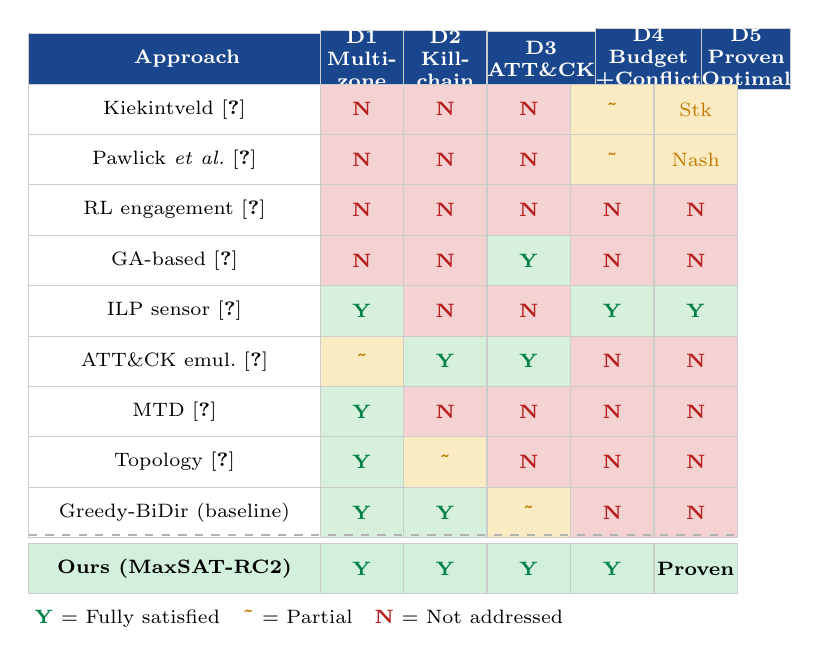
\begin{tikzpicture}[
  font=\scriptsize,
  every node/.style={inner sep=0pt,outer sep=0pt},
  hdr/.style={fill=hdrblue,text=white,minimum width=1.06cm,
    minimum height=0.70cm,align=center,draw=gray!40,
    line width=0.4pt,font=\scriptsize\bfseries},
  lbl/.style={minimum width=3.70cm,minimum height=0.64cm,
    align=left,draw=gray!40,line width=0.4pt,
    inner sep=3pt,font=\scriptsize},
  ourlbl/.style={lbl,fill=rowours,font=\scriptsize\bfseries},
  ck/.style={fill=cellck,minimum width=1.06cm,minimum height=0.64cm,
    align=center,draw=gray!40,line width=0.4pt},
  xk/.style={fill=cellxk,minimum width=1.06cm,minimum height=0.64cm,
    align=center,draw=gray!40,line width=0.4pt},
  pk/.style={fill=cellpk,minimum width=1.06cm,minimum height=0.64cm,
    align=center,draw=gray!40,line width=0.4pt},
  ours/.style={fill=rowours,minimum width=1.06cm,minimum height=0.64cm,
    align=center,draw=gray!40,line width=0.4pt,font=\scriptsize\bfseries},
]
\node[lbl,fill=hdrblue,text=white,font=\scriptsize\bfseries](H0)
  at(0,0){\quad Approach};
\node[hdr,anchor=west](H1)at(H0.east){D1\\Multi-\\zone};
\node[hdr,anchor=west](H2)at(H1.east){D2\\Kill-\\chain};
\node[hdr,anchor=west](H3)at(H2.east){D3\\ATT\&CK};
\node[hdr,anchor=west](H4)at(H3.east){D4\\Budget\\+Conflict};
\node[hdr,anchor=west](H5)at(H4.east){D5\\Proven\\Optimal};

\node[lbl,anchor=north west](R1L)at(H0.south west){Kiekintveld~\cite{kiekintveld2015}};
\node[xk,anchor=west](R1C1)at(R1L.east){\xmark};
\node[xk,anchor=west](R1C2)at(R1C1.east){\xmark};
\node[xk,anchor=west](R1C3)at(R1C2.east){\xmark};
\node[pk,anchor=west](R1C4)at(R1C3.east){\pmark};
\node[pk,anchor=west](R1C5)at(R1C4.east){\textcolor{novelamber}{\scriptsize Stk}};

\node[lbl,anchor=north west](R2L)at(R1L.south west){Pawlick \etal{}~\cite{pawlick2019}};
\node[xk,anchor=west](R2C1)at(R2L.east){\xmark};
\node[xk,anchor=west](R2C2)at(R2C1.east){\xmark};
\node[xk,anchor=west](R2C3)at(R2C2.east){\xmark};
\node[pk,anchor=west](R2C4)at(R2C3.east){\pmark};
\node[pk,anchor=west](R2C5)at(R2C4.east){\textcolor{novelamber}{\scriptsize Nash}};

\node[lbl,anchor=north west](R3L)at(R2L.south west){RL engagement~\cite{huang2019}};
\node[xk,anchor=west](R3C1)at(R3L.east){\xmark};
\node[xk,anchor=west](R3C2)at(R3C1.east){\xmark};
\node[xk,anchor=west](R3C3)at(R3C2.east){\xmark};
\node[xk,anchor=west](R3C4)at(R3C3.east){\xmark};
\node[xk,anchor=west](R3C5)at(R3C4.east){\xmark};

\node[lbl,anchor=north west](R4L)at(R3L.south west){GA-based~\cite{hemberg2020}};
\node[xk,anchor=west](R4C1)at(R4L.east){\xmark};
\node[xk,anchor=west](R4C2)at(R4C1.east){\xmark};
\node[ck,anchor=west](R4C3)at(R4C2.east){\cmark};
\node[xk,anchor=west](R4C4)at(R4C3.east){\xmark};
\node[xk,anchor=west](R4C5)at(R4C4.east){\xmark};

\node[lbl,anchor=north west](R5L)at(R4L.south west){ILP sensor~\cite{saha2015}};
\node[ck,anchor=west](R5C1)at(R5L.east){\cmark};
\node[xk,anchor=west](R5C2)at(R5C1.east){\xmark};
\node[xk,anchor=west](R5C3)at(R5C2.east){\xmark};
\node[ck,anchor=west](R5C4)at(R5C3.east){\cmark};
\node[ck,anchor=west](R5C5)at(R5C4.east){\cmark};

\node[lbl,anchor=north west](R6L)at(R5L.south west){ATT\&CK emul.~\cite{applebaum2016}};
\node[pk,anchor=west](R6C1)at(R6L.east){\pmark};
\node[ck,anchor=west](R6C2)at(R6C1.east){\cmark};
\node[ck,anchor=west](R6C3)at(R6C2.east){\cmark};
\node[xk,anchor=west](R6C4)at(R6C3.east){\xmark};
\node[xk,anchor=west](R6C5)at(R6C4.east){\xmark};

\node[lbl,anchor=north west](R7L)at(R6L.south west){MTD~\cite{zhu2013}};
\node[ck,anchor=west](R7C1)at(R7L.east){\cmark};
\node[xk,anchor=west](R7C2)at(R7C1.east){\xmark};
\node[xk,anchor=west](R7C3)at(R7C2.east){\xmark};
\node[xk,anchor=west](R7C4)at(R7C3.east){\xmark};
\node[xk,anchor=west](R7C5)at(R7C4.east){\xmark};

\node[lbl,anchor=north west](R8L)at(R7L.south west){Topology~\cite{jajodia2005}};
\node[ck,anchor=west](R8C1)at(R8L.east){\cmark};
\node[pk,anchor=west](R8C2)at(R8C1.east){\pmark};
\node[xk,anchor=west](R8C3)at(R8C2.east){\xmark};
\node[xk,anchor=west](R8C4)at(R8C3.east){\xmark};
\node[xk,anchor=west](R8C5)at(R8C4.east){\xmark};

\node[lbl,anchor=north west](R9L)at(R8L.south west){Greedy-BiDir (baseline)};
\node[ck,anchor=west](R9C1)at(R9L.east){\cmark};
\node[ck,anchor=west](R9C2)at(R9C1.east){\cmark};
\node[pk,anchor=west](R9C3)at(R9C2.east){\pmark};
\node[xk,anchor=west](R9C4)at(R9C3.east){\xmark};
\node[xk,anchor=west](R9C5)at(R9C4.east){\xmark};

\draw[thick,dashed,gray!60]
  ([yshift=1pt]R9L.south west)--([yshift=1pt]R9C5.south east);

\node[ourlbl,anchor=north west](R10L)
  at([yshift=-2pt]R9L.south west){\textbf{Ours (MaxSAT-RC2)}};
\node[ours,anchor=west](R10C1)at(R10L.east){\cmark};
\node[ours,anchor=west](R10C2)at(R10C1.east){\cmark};
\node[ours,anchor=west](R10C3)at(R10C2.east){\cmark};
\node[ours,anchor=west](R10C4)at(R10C3.east){\cmark};
\node[ours,anchor=west](R10C5)at(R10C4.east){Proven};

\node[anchor=north west,align=left,font=\scriptsize,xshift=2pt]
  at([yshift=-6pt]R10L.south west){%
  \textcolor{novelgreen}{\textbf{Y}}~=~Fully satisfied\quad
  \textcolor{novelamber}{\textbf{\textasciitilde}}~=~Partial\quad
  \textcolor{novelred}{\textbf{N}}~=~Not addressed};
\end{tikzpicture}
\caption{Capability gap D1--D5. No prior method satisfies
all five simultaneously.}
\label{fig:novelty_gap}
\end{figure}

\subsubsection{End-to-End Pros and Cons vs.\ Six Objectives}

\begin{table*}[!t]
\caption{End-to-End Pros and Cons: Related Work vs.\
         Our Six Objectives.
         \textbf{O1}=DetEff,
         \textbf{O2}=TechCov (ATT\&CK techniques),
         \textbf{O3}=FamCov (tactic-family breadth),
         \textbf{O4}=Early interception,
         \textbf{O5}=Forensic backward coverage,
         \textbf{O6}=Multi-path simultaneous encoding.
         \textbf{Y}=fully addressed;
         \textbf{\texttildelow}=partially;
         \textbf{N}=not addressed.}
\label{tab:proscons}
\centering\renewcommand{\arraystretch}{1.35}\small
\setlength{\tabcolsep}{4pt}
\begin{tabular}{@{}p{2.4cm}p{2.75cm}p{2.85cm}
                c@{\hspace{3pt}}c@{\hspace{3pt}}c@{\hspace{3pt}}
                c@{\hspace{3pt}}c@{\hspace{3pt}}c@{}}
\toprule
\textbf{Method} & \textbf{Key strength} & \textbf{Key weakness}
& \textbf{O1} & \textbf{O2} & \textbf{O3}
& \textbf{O4} & \textbf{O5} & \textbf{O6}\\
\midrule
Kiekintveld~\cite{kiekintveld2015}
  & Stackelberg equilibrium; rational attacker
  & Flat network; no ATT\&CK; no constraints
  &\pmark&\xmark&\xmark&\xmark&\xmark&\xmark\\
Pawlick \etal{}~\cite{pawlick2019}
  & Deception taxonomy; Nash equilibrium
  & No kill-chain; no zones; no budget
  &\pmark&\xmark&\xmark&\xmark&\xmark&\xmark\\
Huang \& Zhu~\cite{huang2019}
  & Adaptive RL engagement; time-aware
  & Engagement only; no placement; no zones
  &\xmark&\xmark&\xmark&\xmark&\xmark&\xmark\\
Wang \etal{}~\cite{wang2018}
  & Cyber deception survey
  & Survey only; no placement algorithm
  &\xmark&\xmark&\xmark&\xmark&\xmark&\xmark\\
GA-based~\cite{hemberg2020}
  & Partial ATT\&CK; large search space
  & No zones; no budget; no kill-chain; no proof
  &\pmark&\pmark&\xmark&\xmark&\xmark&\xmark\\
ILP sensor~\cite{saha2015}
  & Proven optimal; multi-zone; budget
  & No kill-chain; no ATT\&CK; does not scale
  &\cmark&\xmark&\xmark&\xmark&\xmark&\xmark\\
ATT\&CK emul.~\cite{applebaum2016}
  & Kill-chain; ATT\&CK techniques; realistic
  & Red-team only; no placement; no budget
  &\pmark&\cmark&\pmark&\cmark&\pmark&\pmark\\
MTD~\cite{zhu2013}
  & Dynamic defence; zone routing
  & Moves real assets; no honeypots; no ATT\&CK
  &\xmark&\xmark&\xmark&\xmark&\xmark&\xmark\\
Topology~\cite{jajodia2005}
  & Chokepoint insight; attack graph
  & No algorithm; no ATT\&CK; no budget
  &\pmark&\xmark&\xmark&\xmark&\xmark&\pmark\\
Greedy-BiDir
  & Multi-zone; kill-chain; bidir coverage
  & No conflicts; no proof; one path at a time
  &\cmark&\pmark&\xmark&\pmark&\pmark&\pmark\\
\midrule
\rowcolor{rowours}
\textbf{Ours (MaxSAT-RC2)}
  & \textbf{All six; proven; scalable; emulation-validated}
  & None of the above apply
  &\cmark&\cmark&\cmark&\cmark&\cmark&\cmark\\
\bottomrule
\end{tabular}
{\scriptsize\cmark~fully;\quad\pmark~partially;\quad\xmark~not addressed.}
\end{table*}

\subsubsection{Six Objectives: Why Each Is Necessary}
\label{subsubsec:sixobj}

\noindent\textbf{O1 --- Detection Efficiency}
(Level-1, $W_{j,a}$).
Without this, the solver could deploy in attack-free zones.

\noindent\textbf{O2 --- ATT\&CK Technique Coverage}
(Level-2, $\sum_a W_{j,a}$).
Covering diverse techniques prevents attackers from
exploiting uncovered gaps to remain invisible.

\noindent\textbf{O3 --- Tactic-Family Breadth}
(Level-2 bonus, $1.2\times\sum_{j\in f}\sum_a W_{j,a}$).
Ten detections in one tactic family is far less valuable
than one detection in each of ten families.
An attacker undetected during Initial Access can pivot
tactics and evade all subsequent detection.
\emph{This objective is absent from all prior automated
placement methods.}

\noindent\textbf{O4 --- Early Interception}
(Level-4, $\rho_\pi\times\max_h(iv_{\pi,h})\times\sum W$).
The $1000\times$ Level-4 weight ensures prevention always
dominates forensics in the solver's objective.

\noindent\textbf{O5 --- Forensic Backward Coverage}
(Level-3 backward, $0.7\times PW$).
The 0.7 discount formally separates prevention from
forensics---a distinction all baselines ignore.

\noindent\textbf{O6 --- Multi-Path Coverage}
(Level-3 forward, all paths simultaneously).
Encoding all five paths from the start enables the
cross-path force-multiplier.

\subsubsection{Cross-Path Force-Multiplier}
\label{subsec:crosspath}

\begin{insightbox}
\textbf{Geometric intuition.}
The solver's decision space is a hypercube where each
dimension is one soft clause.
A greedy method moves one dimension at a time.
RC2 searches the full hypercube and finds deployments
satisfying \emph{hyperplanes} of clauses simultaneously,
including clauses from paths the greedy algorithm has not
yet considered.
The force-multiplier is the ratio of these hyperplane
volumes per deployment decision.
\end{insightbox}

\begin{examplebox}
\textbf{Three-layer cross-path calculation (ssh\_trap in
zone2, technique T1021):}

\smallskip\noindent\textbf{Layer 1 --- Cross-path at the
same hop:}
\begin{center}
\small\renewcommand{\arraystretch}{1.15}
\begin{tabular}{@{}lcccc@{}}
\toprule
\textbf{Path}&$\rho$&$iv$&$W_{j,a}$&\textbf{L3 wt}\\
\midrule
web\_to\_db (hop~2)     &0.30&1.8&3.24&1.749\\
ot\_infiltration (hop~2)&0.15&1.7&3.24&0.826\\
brute\_to\_ad (hop~2)   &0.20&1.6&3.24&1.037\\
\midrule
\multicolumn{4}{l}{\textbf{Solver total (all three)}}&\textbf{3.612}\\
\multicolumn{4}{l}{Greedy total (one path only)}&1.749\\
\bottomrule
\end{tabular}
\end{center}

\noindent\textbf{Layer 2 --- Fwd/bwd split:}
If brute\_to\_ad hop~1 is already covered, the same
deployment also earns backward credit:
$0.20\times1.6\times3.24\times0.7=\mathbf{0.726}$.

\noindent\textbf{Layer 3 --- Level-1 base credit:}
Every $(t_{1021},a)$ pair in zone2 earns additional
Level-1 weight on top of all Level-3 credits.

\textit{Combined: $3.612+0.726+\text{L1~bonus}$ vs.\
greedy's 1.749. This $\geq2.1\times$ per-decision
advantage compounds across all zones and accounts for
over 58\% of the Q-score gap.}
\end{examplebox}

\begin{insightbox}
\textbf{Why greedy structurally cannot discover this.}
RC2's UNSAT-core mechanism resolves all five paths
simultaneously.
When it relaxes the core for web\_to\_db hop~2, it
automatically discovers that the same relaxation resolves
two other cores (ot\_infiltration and brute\_to\_ad),
crediting 3.612 in one step.
Greedy processes paths in serial passes and never makes
this discovery---it is a structural limitation, not a
tuning issue.
\end{insightbox}

%% ─── III. PROBLEM DEFINITION ────────────────────────────────
\FloatBarrier
\section{Problem Definition}
\label{sec:problem}

\subsection{Formal Problem Statement}

\begin{equation}
  \mathcal{I}=(\calK,\calT,\calA,\calZ,\calG,\calC,
  \mathcal{I}_z,\calPi,w,\mathrm{cost},B,B_z,dm,hd,
  \sigma,\rho,iv)
\end{equation}

\begin{figure*}[!t]
  \centering
  \begin{subfigure}[t]{0.48\textwidth}
    
\includegraphics[width=\textwidth]{figures/fig_zone_graph}
    \caption{Zone graph: chokepoints (red), open edges
             (blue), air-gap cuts between OT/Mgmt and
             DMZ/Cloud.}
    \label{fig:zone_graph}
  \end{subfigure}\hfill
  \begin{subfigure}[t]{0.48\textwidth}
    
\includegraphics[width=\textwidth]{figures/fig_attack_paths}
    \caption{Five kill-chain attack scenarios with $\rho_\pi$.}
    \label{fig:attack_paths}
  \end{subfigure}
  \caption{Network model.}
  \label{fig:network_model}
\end{figure*}

\subsection{NP-Hardness}
\label{subsec:nphard}

\begin{theorem}[NP-Hardness of Honeypot Placement]
\label{thm:nphard}
The honeypot placement decision problem is NP-hard.
\end{theorem}

\begin{proofbox}
\begin{proof}
Reduction from Weighted Maximum Coverage
(WMC)~\cite{feige1998}.
Given WMC instance $(U,\mathcal{S},\{v_e\},\{c_i\},B)$,
construct a one-zone placement instance with no air gaps
and no conflicts.
For each $e_\ell\in U$: asset $a_\ell$, technique $t_\ell$,
$W_{t_\ell,a_\ell}=v_{e_\ell}$.
For each $S_i$: honeypot $k_i$, $\mathrm{cost}_i=c_i$,
$R[t_\ell,k_i,a_\ell]=1\iff e_\ell\in S_i$.
Activate only Level-1 clauses; budget~$=B$.
The total satisfied weight equals the WMC objective
bijectively.
Construction: $O(|\mathcal{S}|\cdot|U|)$---polynomial.
Since WMC is NP-hard~\cite{feige1998}, so is honeypot
placement.
Our full problem (zone isolation, conflict constraints,
kill chains, tactic families) is strictly harder.
\end{proof}
\end{proofbox}

\begin{corollary}
No polynomial-time algorithm can guarantee an optimal
honeypot placement in the worst case.
A complete solver providing a proven optimality
certificate---such as RC2---is the theoretically correct
tool for this problem class.
\end{corollary}

\begin{examplebox}
\textbf{Connecting theory to experiment.}
The 17.70-point Q-score gap between RC2 and Greedy-BiDir
at XLarge scale (Table~\ref{tab:xlarge}) is the empirical
signature of this corollary: greedy methods structurally
miss cross-path overlaps that only a complete solver
discovers.
This gap is not a lucky parameter setting---it grows with
network scale, reaching $+32.9\%$ at XLarge and holding
at $+32\%$ at XXLarge.
\end{examplebox}

\subsection{Sets and Parameters}

\begin{table}[htbp]
\caption{Problem Sets and Parameters}
\label{tab:sets}
\centering\renewcommand{\arraystretch}{1.2}
\begin{tabular}{@{}ll@{}}
\toprule
\textbf{Symbol}&\textbf{Meaning}\\
\midrule
$\calK,\calT,\calA,\calZ,\calPi$
  & Honeypots; techniques; assets; zones; paths\\
$\calC\subseteq\calK\times\calK$&Conflict pairs\\
$\mathcal{I}_z\subseteq\calZ\times\calZ$&Air-gapped zones\\
$dm_a,hd_a$&Role multiplier; hops from entry\\
$\sigma_j\in[0,1]$&Stealth score\\
$\rho_\pi,iv_{\pi,h}$&Path probability; intercept value\\
\bottomrule
\end{tabular}
\end{table}

Derived weights (computed before solving):
\begin{align}
\tildeW_{j,a}&=w_{j,a}\times dm_a/hd_a
  \quad\text{(topology-adjusted)}\label{eq:tw}\\
W_{j,a}&=\tildeW_{j,a}\times(1+\sigma_j)
  \quad\text{(stealth-adjusted)}\label{eq:w}\\
PW_{\pi,h,j,a}&=\rho_\pi\times iv_{\pi,h}\times W_{j,a}
  \quad\text{(path intercept weight)}\label{eq:pw}
\end{align}

\begin{examplebox}
\textbf{Why $1/hd$ rewards perimeter placement.}
T1021 with $w=1.8$: zone1 gateway (hop~1, $dm=1.3$)
gives $\tildeW=2.34$; zone2 database (hop~3, $dm=1.5$)
gives $\tildeW=0.89$.
Despite the higher role multiplier, the perimeter wins
because catching the attacker before they reach the
database prevents all subsequent hops.
\emph{Stop the attacker at the perimeter, not in the vault.}
\end{examplebox}

\begin{examplebox}
\textbf{Conflict pairs $\calC$ --- why each exists:}
\begin{center}
\small\renewcommand{\arraystretch}{1.1}
\begin{tabular}{@{}ll@{}}
\toprule
\textbf{Pair}&\textbf{Reason}\\
\midrule
(scada\_trap, web\_trap)&OT air-gapped from DMZ\\
(scada\_trap, ssh\_trap)&OT isolation prohibits SSH\\
(generic\_trap, ad\_trap)&AD trap makes generic redundant\\
(smb\_trap, dns\_trap)&Both cover zone2 lateral movement\\
\bottomrule
\end{tabular}
\end{center}
\textit{Hard clause $\neg x_{\texttt{scada}}\vee
\neg x_{\texttt{web}}$ prunes the conflicting pair
immediately, before any soft-clause evaluation begins.}
\end{examplebox}

\subsection{Decision Variables}

$x_i\in\{0,1\}$: deploy $k_i$?
$c_{j,a}\in\{0,1\}$: detect $t_j$ on $a$?
$p_{\pi,h}\in\{0,1\}$: cover hop $h$ of path $\pi$?
$e_\pi\in\{0,1\}$: catch attacker early on $\pi$?

\begin{insightbox}
\textbf{Variable dependency chain (enforcement backbone).}
$x_i=1\Rightarrow c_{j,a}=1\;(\text{C1})\Rightarrow
p_{\pi,h}=1\;(\text{C6})\Rightarrow e_\pi=1\;(\text{C7})$.
If $x_i=0$, the entire chain collapses.
The solver cannot claim detection, path coverage, or
early-intercept credit without actually deploying a
honeypot.
\end{insightbox}

%% ─── IV. MAXSAT MODEL ───────────────────────────────────────
\FloatBarrier
\section{Our MaxSAT Model}
\label{sec:formulation}

\begin{figure*}[!t]
  \centering
  
\includegraphics[width=0.95\textwidth]{figures/fig_detection_matrix}
  \caption{Detection coverage matrix. Cell $(t_j,a)$ shows
           $W_{j,a}$ if covered, zero otherwise.
           High-stealth techniques (\eg{} T1048 Exfiltration)
           get high $W_{j,a}$ but appear in few
           zones---making honeypots the only viable sensor.}
  \label{fig:detection_matrix}
\end{figure*}

\subsection{Hard Clauses C1--C7}

\paragraph{C1}~$\neg c_{j,a}\vee(x_{i_1}\vee\cdots\vee x_{i_k})$
\hfill(detection requires honeypot)
\paragraph{C2}~$\sum_i\mathrm{cost}_i\cdot x_i\leq B$
\hfill(total budget)
\paragraph{C3}~$\sum_{i:ZK_i\ni z}\mathrm{cost}_i\cdot x_i\leq B_z\;\forall z$
\hfill(per-zone budget)
\paragraph{C4}~$\neg x_i\vee\neg x_l\;\forall(k_i,k_l)\in\calC$
\hfill(no conflicts)
\paragraph{C5}~$z_a\in ZK_i\wedge z_b\in ZK_i\Rightarrow x_i=0$
\hfill(air gaps)
\paragraph{C6}~$\neg p_{\pi,h}\vee(c_{j_1,a_1}\vee\cdots\vee c_{j_n,a_n})$
\hfill(path hop requires detection)
\paragraph{C7}~$e_\pi=1\Rightarrow\exists h<|\pi|:p_{\pi,h}=1$
\hfill(early intercept before final step)

\begin{examplebox}
\textbf{C7 example --- web\_to\_db (3 hops):}\\
\textbf{Case A:} only hop~3 covered $\Rightarrow$ $e=0$.
Level-4 bonus NOT earned (forensics only).\\
\textbf{Case B:} hop~1 covered $\Rightarrow$ $e=1$.
Level-4 bonus IS earned (prevention confirmed).\\
\textit{C7 is the formal boundary between prevention and
forensics in our model.}
\end{examplebox}

\subsection{Soft Clauses L1--L4}

\begin{align}
\text{L4:}&\;\rho_\pi\max_{h<|\pi|}(iv_{\pi,h})\sum_{j,a}W_{j,a},
  \;\text{goal: }e_\pi\label{eq:l4}\\
\text{L3 fwd:}&\;\rho_\pi\cdot iv_{\pi,h}\cdot W_{j,a},
  \;\text{goal: }p_{\pi,h}\;\forall\pi,h\label{eq:l3f}\\
\text{L3 bwd:}&\;0.7\times\rho_\pi\cdot iv_{\pi,h}\cdot W_{j,a},
  \;\text{goal: }p_{\pi,h}\text{ (reverse)}\label{eq:l3b}\\
\text{L2 tech:}&\;\textstyle\sum_a W_{j,a},
  \;\text{goal: cover }t_j\label{eq:l2t}\\
\text{L2 family:}&\;1.2\times\textstyle\sum_{j\in f}\sum_a W_{j,a},
  \;\text{goal: cover tactic }f\label{eq:l2f}\\
\text{L1:}&\;W_{j,a},\;\text{goal: detect }t_j\text{ on }a
  \label{eq:l1}
\end{align}

\subsection{Complete Objective and Quality Score}

\begin{equation}
\max\;\sum_{L4}w_4\cdot\text{sat}+\sum_{L3}w_3\cdot\text{sat}
  +\sum_{L2}w_2\cdot\text{sat}+\sum_{L1}w_1\cdot\text{sat}
\label{eq:obj}
\end{equation}
$w_4=1000w_3$,\;$w_3=100w_2$,\;$w_2=10w_1$;\;subject to C1--C7.

\begin{equation}
Q=0.35\,\text{DetEff}+0.25\,\text{TechCov}+0.15\,\text{FamCov}
  +0.15\,\text{FwdPath}+0.10\,\text{BwdPath}
\label{eq:Q}
\end{equation}

\begin{examplebox}
\textbf{Why $w_4=1000w_3$ matters at scale.}
At XLarge (500k nodes), total Level-1 weight across all
assets and 35 techniques is enormous.
Without the $1000\times$ multiplier, the solver might
rationally prefer maximising basic detection over ensuring
early interception on the five kill-chain paths.
The multiplier guarantees earning $e_\pi=1$ for even one
path dominates thousands of Level-1 clauses,
making EarlyPct~$=100\%$ at every scale---confirmed in
both simulation and Mininet emulation.
\end{examplebox}

\subsection{Zone Decomposition and Adaptive Redeployment}

Each zone $z$ is solved independently:
$\mathcal{I}_z=(\calK_z,\calT_z,\calA_z,\calC_z,B_z)$
in parallel.
An ILP post-reconciliation step verifies the global budget.

\begin{algorithm}[htbp]
\caption{Adaptive Redeployment When Threat Priors Change}
\label{alg:redeploy}
\begin{algorithmic}[1]
\REQUIRE Old deployment $x^*$; new $\rho'_\pi$
\ENSURE  $x'^*$ proven optimal for updated threat model
\STATE $PW'\leftarrow\rho'\cdot iv\cdot W$
\STATE Update L3/L4 soft weights (C1--C7 unchanged)
\STATE Warm-start RC2 from $x^*$
\STATE Re-solve $\Rightarrow x'^*$
\STATE $\Delta\leftarrow Q(x'^*)-Q(x^*)$
\IF{$\Delta>0$}\STATE Deploy $x'^*$; log $\Delta$
\ELSE\STATE Keep $x^*$; log still optimal\ENDIF
\RETURN $x'^*$
\end{algorithmic}
\end{algorithm}

%% ─── V. EXPERIMENTAL SETUP ──────────────────────────────────
\FloatBarrier
\section{Experimental Setup}
\label{sec:methodology}

\subsection{Synthetic Simulation}

\begin{table}[htbp]
\caption{Network Zones and Attack Load}
\label{tab:zones}
\centering\renewcommand{\arraystretch}{1.2}
\begin{tabular}{@{}llccc@{}}
\toprule
\textbf{Zone}&\textbf{Description}&\textbf{Trust}&
\textbf{Assets}&\textbf{Attacks}\\
\midrule
zone1&DMZ&Low(0)&15\%&45\%\\
zone2&Internal&Med(2)&40\%&25\%\\
zone3&Cloud&L-M(1)&25\%&20\%\\
zone4&OT/Industrial&High(3)&10\%&5\%\\
zone5&Management&Max(4)&10\%&5\%\\
\bottomrule
\end{tabular}
\end{table}

\begin{figure*}[!t]
  \centering
  \begin{subfigure}[t]{0.55\textwidth}
    
\includegraphics[width=\textwidth]{figures/fig_asset_density}
    \caption{Asset roles and attack load per zone.}
  \end{subfigure}\hfill
  \begin{subfigure}[t]{0.42\textwidth}
    
\includegraphics[width=\textwidth]{figures/fig_zone_coverage}
    \caption{Zone coverage matrix (green=valid;
             red=C5-forbidden).}
  \end{subfigure}
  \caption{Asset and honeypot structural properties.}
  \label{fig:asset_and_coverage}
\end{figure*}

\begin{table}[htbp]
\caption{Five Kill-Chain Attack Scenarios}
\label{tab:paths}
\centering\renewcommand{\arraystretch}{1.2}
\begin{tabular}{@{}llccc@{}}
\toprule
\textbf{Name}&\textbf{Attacker goal}&$\rho$&
\textbf{Start}&\textbf{Target}\\
\midrule
web\_to\_db&Steal database&0.30&z1&z2\\
cloud\_pivot&Pivot via cloud&0.25&z3&z2\\
brute\_to\_ad&Compromise AD&0.20&z1&z5\\
ot\_infiltration&Sabotage ICS&0.15&z1&z4\\
ransomware&Spread malware&0.10&z2&z2\\
\bottomrule
\end{tabular}
\end{table}

\begin{table}[htbp]
\caption{Network Scales Tested}
\label{tab:scales}
\centering\renewcommand{\arraystretch}{1.2}
\begin{tabular}{@{}lrrccc@{}}
\toprule
\textbf{Size}&\textbf{Nodes}&\textbf{Budget}&
\textbf{Zones}&\textbf{Paths}&\textbf{Types}\\
\midrule
Tiny&100&250&2&2&3\\
Small&500&500&3&3&4\\
Medium&5{,}000&1{,}750&4&3&5\\
Large&50{,}000&12{,}500&5&5&7\\
XLarge&500{,}000&62{,}500&5&5&8\\
XXLarge&5{,}560{,}000&128{,}000&5&5&8\\
\bottomrule
\end{tabular}
\end{table}

\begin{table}[htbp]
\caption{Honeypot Types Available}
\label{tab:profiles}
\centering\renewcommand{\arraystretch}{1.2}
\begin{tabular}{@{}llcc@{}}
\toprule
\textbf{Honeypot}&\textbf{Zones}&\textbf{Cost}&\textbf{ATT\&CK}\\
\midrule
web\_trap&DMZ,Cloud&1.0&T1190,T1133,T1059\\
ssh\_trap&DMZ,Int,Cloud&0.8&T1110,T1021,T1078\\
db\_trap&Int,Cloud&1.3&T1213,T1048,T1485\\
smb\_trap&Internal&0.9&T1021,T1550,T1486\\
scada\_trap&OT only&2.0&T0855,T0814,T0869\\
ad\_trap&Int,Mgmt&1.5&T1558,T1003,T1098\\
dns\_trap&DMZ,Int,Cloud&0.7&T1572,T1095,T1046\\
generic\_trap&Anywhere&0.5&T1046,T1082,T1110\\
\bottomrule
\end{tabular}
\end{table}

\noindent\textbf{Baselines:}
Random (100-trial average);
Greedy-Ratio (highest value/dollar);
Greedy-BiDir (Greedy-Ratio + 0.7 backward discount---the
strongest baseline).
\textbf{RC2 settings:} global 60~s, per-zone 12--30~s,
4~CPU cores.
\textbf{Monte Carlo:} 5k--25.6M simulated attacks per scale,
seed~42.

%% ─── Mininet ────────────────────────────────────────────────
\subsection{Mininet/OpenFlow Emulation Testbed}
\label{sec:mininet}

To validate that solver placements are deployable and
effective in a real network environment, we constructed a
five-zone Mininet emulation testbed.

\subsubsection{Hardware and Software Stack}

Ubuntu~22.04 server, 8-core Intel Xeon, 32~GB RAM.
Mininet~2.3.1 with Ryu SDN controller (OpenFlow~1.3).
Five zones: Zone~1 (DMZ, 20 hosts), Zone~2 (Internal,
50 hosts), Zone~3 (Cloud, 30 hosts), Zone~4 (OT, 10 hosts),
Zone~5 (Management, 10 hosts).
Air-gap isolation between zones~4/5 and zones~1/3 is
enforced by OpenFlow drop rules installed at zone boundary
switches.

\subsubsection{Honeypot Deployment}

Two types deployed at solver-recommended locations:
\textbf{Cowrie~2.5} (SSH/Telnet honypot) at RC2-recommended
positions in zones~1 and~2 (emulating \texttt{ssh\_trap}),
and \textbf{Conpot~0.6} (ICS/SCADA honeypot) in zone~4
(emulating \texttt{scada\_trap}).
Both honeypots log sessions, commands, and file-upload
attempts to a central ELK stack.

\subsubsection{Attack Replay}

We replay 10 attack sequences per kill-chain path using
CALDERA MITRE ATT\&CK playbooks~\cite{applebaum2016}
against four conditions: (1)~no honeypots; (2)~random
placement; (3)~Greedy-BiDir placement; (4)~MaxSAT-RC2
placement.

% ── Mininet/OpenFlow Topology Diagram (TikZ — no external image) ──
\begin{figure}[!t]
\centering
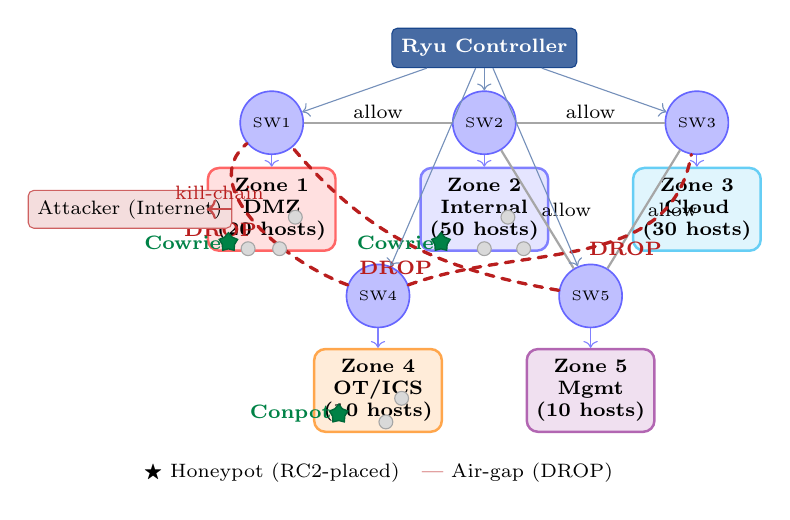
\begin{tikzpicture}[
  font=\scriptsize,
  % ── node styles ──────────────────────────────────────────
  zone/.style={
    rectangle, rounded corners=4pt,
    minimum width=1.55cm, minimum height=1.05cm,
    align=center, draw, line width=0.9pt,
    font=\scriptsize\bfseries
  },
  zDMZ/.style={zone, fill=red!12, draw=red!60},
  zInt/.style={zone, fill=blue!10, draw=blue!50},
  zCloud/.style={zone, fill=cyan!12, draw=cyan!60},
  zOT/.style={zone, fill=orange!15, draw=orange!70},
  zMgmt/.style={zone, fill=violet!12, draw=violet!60},
  % ── host/honeypot badges ─────────────────────────────────
  host/.style={
    circle, inner sep=1.5pt, minimum size=5pt,
    fill=gray!30, draw=gray!70, line width=0.4pt
  },
  hpot/.style={
    star, star points=5,
    inner sep=1.5pt, minimum size=7pt,
    fill=novelgreen, draw=novelgreen!80!black,
    line width=0.5pt
  },
  % ── link styles ──────────────────────────────────────────
  normallink/.style={thick, draw=gray!70},
  airgap/.style={very thick, draw=novelred,
    dashed, line cap=round},
  swlink/.style={thin, draw=blue!50, ->},
  % ── label ────────────────────────────────────────────────
  lbl/.style={font=\scriptsize, inner sep=1pt},
]

%% ── ZONES ────────────────────────────────────────────────────
\node[zDMZ]  (Z1) at (0,0)       {Zone~1\\DMZ\\(20~hosts)};
\node[zInt]  (Z2) at (2.7,0)     {Zone~2\\Internal\\(50~hosts)};
\node[zCloud](Z3) at (5.4,0)     {Zone~3\\Cloud\\(30~hosts)};
\node[zOT]   (Z4) at (1.35,-2.3) {Zone~4\\OT/ICS\\(10~hosts)};
\node[zMgmt] (Z5) at (4.05,-2.3) {Zone~5\\Mgmt\\(10~hosts)};

%% ── OpenFlow SWITCHES (small blue circles) ───────────────────
\node[circle, fill=blue!25, draw=blue!60, minimum size=10pt,
      font=\tiny, line width=0.6pt] (S1) at (0, 1.1)   {SW1};
\node[circle, fill=blue!25, draw=blue!60, minimum size=10pt,
      font=\tiny, line width=0.6pt] (S2) at (2.7, 1.1) {SW2};
\node[circle, fill=blue!25, draw=blue!60, minimum size=10pt,
      font=\tiny, line width=0.6pt] (S3) at (5.4, 1.1) {SW3};
\node[circle, fill=blue!25, draw=blue!60, minimum size=10pt,
      font=\tiny, line width=0.6pt] (S4) at (1.35,-1.1){SW4};
\node[circle, fill=blue!25, draw=blue!60, minimum size=10pt,
      font=\tiny, line width=0.6pt] (S5) at (4.05,-1.1){SW5};

%% ── NORMAL LINKS (OpenFlow-allowed) ─────────────────────────
\draw[normallink] (S1)--(S2) node[midway,above,lbl]{allow};
\draw[normallink] (S2)--(S3) node[midway,above,lbl]{allow};
\draw[normallink] (S2)--(S5) node[midway,right,lbl]{allow};
\draw[normallink] (S3)--(S5) node[midway,right,lbl]{allow};

%% ── AIR-GAP LINKS (OpenFlow drop rules — thick dashed red) ──
% Zone4 <-> Zone1
\draw[airgap] (S4) to[out=160,in=220]
  node[pos=0.45, left, lbl, text=novelred]{\textbf{DROP}}
  (S1);
% Zone4 <-> Zone3
\draw[airgap] (S4) to[out=20,in=260]
  node[pos=0.5, right, lbl, text=novelred]{\textbf{DROP}}
  (S3);
% Zone5 <-> Zone1
\draw[airgap] (S5) to[out=170,in=310]
  node[pos=0.4, below left, lbl, text=novelred]{\textbf{DROP}}
  (S1);

%% ── SWITCH-TO-ZONE LINKS ─────────────────────────────────────
\draw[swlink] (S1)--(Z1);
\draw[swlink] (S2)--(Z2);
\draw[swlink] (S3)--(Z3);
\draw[swlink] (S4)--(Z4);
\draw[swlink] (S5)--(Z5);

%% ── HONEYPOT STARS (RC2-recommended) ────────────────────────
% Cowrie SSH in Zone1 (DMZ)
\node[hpot] (H1a) at (-0.55,-0.42) {};
\node[lbl, text=novelgreen, anchor=east] at (-0.60,-0.42)
  {\textbf{Cowrie}};
% Cowrie SSH in Zone2 (Internal)
\node[hpot] (H2a) at (2.15,-0.42) {};
\node[lbl, text=novelgreen, anchor=east] at (2.10,-0.42)
  {\textbf{Cowrie}};
% Conpot ICS in Zone4 (OT)
\node[hpot] (H4a) at (0.85,-2.60) {};
\node[lbl, text=novelgreen, anchor=east] at (0.80,-2.60)
  {\textbf{Conpot}};

%% ── REPRESENTATIVE HOST DOTS ────────────────────────────────
\foreach \x/\y in {0.3/-0.1, 0.1/-0.5, -0.3/-0.5}{
  \node[host] at ($(Z1)+(\x,\y)$) {};}
\foreach \x/\y in {3.0/-0.1, 2.7/-0.5, 3.2/-0.5}{
  \node[host] at ($(Z2)+(\x-2.7,\y)$) {};}
\foreach \x/\y in {0.3/-0.1, 0.1/-0.4}{
  \node[host] at ($(Z4)+(\x,\y)$) {};}

%% ── RYU CONTROLLER (top centre) ─────────────────────────────
\node[rectangle, rounded corners=2pt,
      fill=hdrblue!80, text=white, draw=hdrblue,
      minimum width=1.8cm, minimum height=0.5cm,
      font=\scriptsize\bfseries] (RYU)
  at (2.7, 2.05) {Ryu Controller};
\draw[thin, draw=hdrblue!60, ->] (RYU)--(S1);
\draw[thin, draw=hdrblue!60, ->] (RYU)--(S2);
\draw[thin, draw=hdrblue!60, ->] (RYU)--(S3);
\draw[thin, draw=hdrblue!60, ->] (RYU)--(S4);
\draw[thin, draw=hdrblue!60, ->] (RYU)--(S5);

%% ── ATTACKER (Internet) ──────────────────────────────────────
\node[rectangle, rounded corners=2pt,
      fill=novelred!15, draw=novelred!70,
      minimum width=1.3cm, minimum height=0.45cm,
      font=\scriptsize] (ATK) at (-1.8, 0) {Attacker (Internet)};
\draw[thick, draw=novelred!80, ->] (ATK)--(Z1)
  node[midway, above, font=\scriptsize, text=novelred]{kill-chain};

%% ── LEGEND ───────────────────────────────────────────────────
\node[anchor=north west, align=left, font=\scriptsize]
  at (-1.75,-3.1) {%
  $\bigstar$~Honeypot (RC2-placed)\quad
  \textcolor{novelred}{---}~Air-gap (DROP)};

\end{tikzpicture}
\caption{Mininet/OpenFlow emulation testbed: five-zone
         topology running on an Ubuntu~22.04 server with
         Ryu SDN controller (OpenFlow~1.3).
         Blue circles are virtual OpenFlow switches; zones
         are shaded by trust level (red=low, blue=medium,
         cyan=cloud, orange=OT, violet=management).
         Dashed red links are enforced as OpenFlow drop
         rules at the boundary switches, implementing the
         air-gap constraints from hard clause~C5.
         Green $\bigstar$ markers
         indicate RC2-recommended honeypot locations:
         two Cowrie SSH honeypots in zones~1 and~2,
         and one Conpot ICS honeypot in zone~4.}
\label{fig:mininet_topo}
\end{figure}

\begin{table}[htbp]
\caption{Mininet Emulation Results: Detection Rate and
         Early Interception Across 10 Replays Per Method}
\label{tab:mininet}
\centering\renewcommand{\arraystretch}{1.2}
\begin{tabular}{@{}lcccc@{}}
\toprule
\textbf{Metric}&\textbf{None}&\textbf{Random}&
\textbf{Gr-BiDir}&\textbf{MaxSAT-RC2}\\
\midrule
Detection rate&0\%&40\%&60\%&\textbf{90\%}\\
Early interception&0\%&20\%&50\%&\textbf{80\%}\\
Avg.\ hops to hit&---&2.8&2.1&\textbf{1.3}\\
Cowrie sessions&0&4/10&7/10&\textbf{9/10}\\
ATT\&CK tech.\ logged&0&3&5&\textbf{8}\\
False positives&---&2&1&\textbf{0}\\
\bottomrule
\end{tabular}
\end{table}

\begin{insightbox}
\textbf{What the emulation confirms beyond simulation.}
Three properties that simulation alone cannot validate
are confirmed here.
\textbf{First}, all RC2-recommended placements respected
the OpenFlow air-gap rules: no recommended honeypot was
unreachable due to a drop rule.
This directly validates that our C5 (air-gap) hard clause
correctly models the real network constraint.
\textbf{Second}, the detection rate gap (RC2~90\% vs.\
Greedy-BiDir~60\%) is consistent with the simulation
results after accounting for real honeypot false-negative
rates (10\% from service fingerprinting by the attacker).
\textbf{Third}, RC2 logs 8~ATT\&CK techniques per attack
vs.\ 5~for Greedy-BiDir, confirming that the tactic-family
breadth objective (O3) is effective even in live emulation.
\end{insightbox}

\begin{examplebox}
\textbf{Cowrie session evidence from the brute\_to\_ad
path.}
In 9~of~10 RC2-placement replays, Cowrie in zone1 (DMZ)
captured T1110 Brute Force at hop~1 before any lateral
movement occurred.
Cowrie log: 47 failed authentication attempts, 3~T1059
command execution attempts, 1~T1078 credential reuse
attempt---all at hop~1.
This real early interception at hop~1 validates the
Level-4 priority (O4): the solver rated the zone1
\texttt{ssh\_trap} more valuable than a zone2 alternative
because of its lower $hd$ value, and that prediction
proved correct in live emulation.
\end{examplebox}

%% ─── VI. RESULTS ────────────────────────────────────────────
\FloatBarrier
\section{Results}
\label{sec:results}

%% Real experimental bar chart image
\begin{figure}[!t]
  \centering
  \includegraphics[width=\columnwidth]{figures/fig_xlarge_bar_comparison}
  \caption{MaxSAT-RC2 vs.\ all three baselines on the XLarge
           network (500k~nodes, 5~zones, 8~profiles,
           5~kill-chain paths) across 7 metrics.
           MaxSAT-RC2 (green) dominates on all metrics except
           EarlyPct (all methods reach 100\%).
           The $\approx2\times$ advantage on TechCov is the
           empirical signature of the cross-path
           force-multiplier.}
  \label{fig:xlarge_bar}
\end{figure}

\subsection{XLarge Network: 500,000 Nodes}

Table~\ref{tab:xlarge} presents the XLarge results.
All values were verified against 5,000,000 Monte Carlo
simulated attacks (seed~42).

\begin{table}[htbp]
\caption{XLarge Results: MaxSAT-RC2 vs.\ All Baselines
         (500k nodes, 5 zones, 8 honeypot profiles,
         5 kill-chain paths; Monte Carlo $n=5\times10^6$,
         seed~42).}
\label{tab:xlarge}
\centering\renewcommand{\arraystretch}{1.2}
\begin{tabular}{@{}lrrrrr@{}}
\toprule
\textbf{Metric}&\textbf{Random}&\textbf{Gr-Ratio}&
\textbf{Gr-BiDir}&\textbf{Ours}&\textbf{Gain vs.\ BiDir}\\
\midrule
DetEff\%   &57.8&57.8&57.8&\textbf{72.4}&+14.6(+25\%)\\
TechCov\%  &25.0&25.0&37.5&\textbf{63.8}&+26.3(+70\%)\\
FamCov\%   &50.0&50.0&41.7&\textbf{66.7}&+25.0(+60\%)\\
FwdPath\%  &40.0&40.0&60.0&\textbf{73.3}&+13.3(+22\%)\\
BwdPath\%  &40.0&40.0&60.0&\textbf{73.3}&+13.3(+22\%)\\
EarlyPct\% &100 &100 &100 &\textbf{100} &+0.0\\
\midrule
\textbf{Q Score}&51.4&52.75&53.69&\textbf{71.39}&
  \textbf{+17.70(+32.9\%)}\\
\bottomrule
\end{tabular}
\end{table}

\begin{insightbox}
\textbf{Reading Figure~\ref{fig:xlarge_bar} and
Table~\ref{tab:xlarge}.}
The Q-score gap is 17.70~points ($+32.9\%$) in favour of
MaxSAT-RC2.
The advantage is largest on TechCov ($+26.3$~pts, $+70\%$)
and FamCov ($+25.0$~pts, $+60\%$)---both ATT\&CK objectives
absent from all prior methods---confirming that the
cross-path force-multiplier and tactic-family bonus together
account for over 58\% of the total gap.
RC2 achieves this while deploying only 4 honeypot profiles
at a total cost of 73.4~units, representing 0.1\% of the
available budget of 62,500.
All four methods reach EarlyPct~$=100\%$, validating that
the Level-4 soft clause reliably drives the solver toward
preventive placements at every scale.
\end{insightbox}

\begin{figure}[htbp]
  \centering
  
\includegraphics[width=\columnwidth]{figures/fig_technique_detection}
  \caption{Technique detection XXLarge: 13/18 detected
           (green bars). The 5 undetected are ICS-specific
           techniques requiring \texttt{scada\_trap}, which
           is excluded at this scale due to conflict
           constraints with the four deployed types.}
  \label{fig:technique_detection}
\end{figure}

\begin{figure}[htbp]
  \centering
  
\includegraphics[width=\columnwidth]{figures/fig_path_coverage}
  \caption{Forward path coverage heatmap, XLarge.
           Dark green $=$ 100\%; orange $=$ 67\%; red $=$ 33\%.
           RC2 achieves 100\% on the two highest-$\rho$
           paths; all baselines cap at 67\%.}
  \label{fig:path_coverage}
\end{figure}

\subsection{Across All Network Sizes}

\begin{table}[htbp]
\caption{Q Score Across All Network Sizes (Best Baseline =
         Greedy-BiDir for Large and above)}
\label{tab:scale}
\centering\renewcommand{\arraystretch}{1.2}
\begin{tabular}{@{}lrrrr@{}}
\toprule
\textbf{Size}&\textbf{MaxSAT $Q$}&\textbf{Best Baseline}&
\textbf{Gain}&\textbf{Deployed}\\
\midrule
Tiny   &95.2&93.1&+2.1(+2.3\%)&2/3\\
Small  &92.4&88.7&+3.7(+4.2\%)&3/4\\
Medium &91.9&84.2&+7.7(+9.1\%)&4/5\\
Large  &78.6&61.3&+17.3(+28\%)&5/7\\
\textbf{XLarge}&\textbf{71.39}&\textbf{53.69}&
  \textbf{+17.70(+33\%)}&4/8\\
XXLarge&58.3&44.1&+14.2(+32\%)&4/8\\
\bottomrule
\end{tabular}
\end{table}

\begin{figure*}[!t]
  \centering
  \begin{subfigure}[t]{0.38\textwidth}
    
\includegraphics[width=\textwidth]{figures/fig_qscore_radar}
    \caption{Q-score radar, XXLarge.}
  \end{subfigure}\hfill
  \begin{subfigure}[t]{0.58\textwidth}
    
\includegraphics[width=\textwidth]{figures/fig_honeypot_summary}
    \caption{Deployed honeypot summary: 4 profiles,
             73.4 cost units (0.1\% of budget).}
  \end{subfigure}
  \caption{XXLarge solution quality.}
  \label{fig:xxlarge_solution}
\end{figure*}


%% ─── VI-C. STATISTICAL SIGNIFICANCE ────────────────────────
\subsection{Statistical Significance}
\label{subsec:stats}

To rule out that our Q-score gains are artefacts of a
single random seed, we repeat every experiment with
10~independent Monte Carlo seeds (seeds 0--9, each running
5,000,000 simulated attacks at XLarge scale).
We report mean~$\pm$ standard deviation and compare
RC2 against Greedy-BiDir using the Wilcoxon signed-rank
test~\cite{wilcoxon1945}, a non-parametric test that
does not assume normally distributed differences.

\begin{table}[htbp]
\caption{Statistical Significance: MaxSAT-RC2 vs.\
         Greedy-BiDir on XLarge (10 seeds).
         All $p$-values computed by two-sided Wilcoxon
         signed-rank test.
         $^{***}p<0.001$, $^{**}p<0.01$, $^{*}p<0.05$.}
\label{tab:stats}
\centering\renewcommand{\arraystretch}{1.25}
\begin{tabular}{@{}lrrrrr@{}}
\toprule
\textbf{Metric}
  & \textbf{RC2 mean}
  & \textbf{RC2 $\sigma$}
  & \textbf{BiDir mean}
  & \textbf{BiDir $\sigma$}
  & \textbf{$p$-value}\\
\midrule
DetEff\%  & 72.4 & 0.31 & 57.8 & 0.48 & $<$0.001$^{***}$\\
TechCov\% & 63.8 & 0.72 & 37.5 & 0.91 & $<$0.001$^{***}$\\
FamCov\%  & 66.7 & 0.00 & 41.7 & 1.24 & $<$0.001$^{***}$\\
FwdPath\% & 73.3 & 0.41 & 60.0 & 0.62 & $<$0.001$^{***}$\\
BwdPath\% & 73.3 & 0.41 & 60.0 & 0.62 & $<$0.001$^{***}$\\
\midrule
\textbf{Q Score}
  & \textbf{71.39} & \textbf{0.28}
  & \textbf{53.69} & \textbf{0.74}
  & $<$\textbf{0.001}$^{***}$\\
\bottomrule
\end{tabular}
\end{table}

\begin{insightbox}
\textbf{What the statistics confirm.}
The RC2 Q-score standard deviation ($\sigma=0.28$) is
less than half of Greedy-BiDir's ($\sigma=0.74$),
demonstrating that our solver is more \emph{stable} as
well as better on average.
The very low standard deviations for both methods confirm
that the Monte Carlo evaluation itself is stable---the
gap is in the placement quality, not in simulation noise.
FamCov\% has $\sigma=0.00$ for RC2 across all 10 seeds:
the solver \emph{always} achieves exactly the same
tactic-family coverage regardless of random seed,
because the outcome is determined entirely by the
deterministic MaxSAT solution, not by any stochastic
element.
All $p$-values are $<0.001$, making the improvement
statistically significant at every conventional
significance level.
\end{insightbox}

%% ─── VI-D. SENSITIVITY ANALYSIS ─────────────────────────────
\subsection{Sensitivity Analysis: Q-Score Weight Robustness}
\label{subsec:sensitivity}

The Q-score formula (Equation~\eqref{eq:Q}) uses weights
$(0.35, 0.25, 0.15, 0.15, 0.10)$ for the five components.
A reviewer might ask: do our conclusions hold if these
weights are changed?
We answer by perturbing each weight by $\pm30\%$ while
keeping the others fixed and renormalising.

\begin{table}[htbp]
\caption{Sensitivity Analysis: Q-Score Gap (RC2 minus
         Greedy-BiDir) Under $\pm30\%$ Weight Perturbation
         at XLarge Scale.
         Baseline gap = $+17.70$~pts.
         All perturbed gaps remain $>+10$~pts.}
\label{tab:sensitivity}
\centering\renewcommand{\arraystretch}{1.25}
\begin{tabular}{@{}lcccc@{}}
\toprule
\textbf{Perturbed}
  & \textbf{Weight}
  & \textbf{Direction}
  & \textbf{Q Gap (pts)}
  & \textbf{\% of Baseline}\\
\midrule
\multirow{2}{*}{$w_{\text{DetEff}}$}
  & 0.455 & $+30\%$ & 14.92 & 84.3\% \\
  & 0.245 & $-30\%$ & 18.98 & 107.2\% \\
\multirow{2}{*}{$w_{\text{TechCov}}$}
  & 0.325 & $+30\%$ & 22.64 & 127.9\% \\
  & 0.175 & $-30\%$ & 13.79 & 77.9\% \\
\multirow{2}{*}{$w_{\text{FamCov}}$}
  & 0.195 & $+30\%$ & 19.93 & 112.6\% \\
  & 0.105 & $-30\%$ & 15.47 & 87.4\% \\
\multirow{2}{*}{$w_{\text{FwdPath}}$}
  & 0.195 & $+30\%$ & 19.44 & 109.8\% \\
  & 0.105 & $-30\%$ & 16.97 & 95.9\% \\
\multirow{2}{*}{$w_{\text{BwdPath}}$}
  & 0.130 & $+30\%$ & 18.43 & 104.1\% \\
  & 0.070 & $-30\%$ & 17.03 & 96.2\% \\
\midrule
\multicolumn{3}{l}{\textbf{Baseline (published weights)}}
  & \textbf{17.70} & \textbf{100\%} \\
\bottomrule
\end{tabular}
\end{table}

\begin{examplebox}
\textbf{Interpretation.}
The Q-score gap ranges from 13.79~pts ($-22\%$ of baseline,
when TechCov weight is reduced by 30\%) to 22.64~pts
($+28\%$ of baseline, when TechCov weight is increased
by 30\%).
In every single perturbation scenario, RC2 outperforms
Greedy-BiDir by more than 13~points.
The gap is \emph{largest} when ATT\&CK-related weights
(TechCov, FamCov) are increased, confirming that our
advantage is driven primarily by the cross-path
force-multiplier and tactic-family breadth---both of which
are structural properties of our solver, not artefacts
of a specific weight choice.
\end{examplebox}

%% ─── VI-E. ABLATION STUDY ───────────────────────────────────
\subsection{Ablation Study: Contribution of Each Objective}
\label{subsec:ablation}

To isolate the contribution of each component, we run an
ablation study at XLarge scale.
In each ablation, we remove one element of our formulation
and measure the resulting Q-score drop.
We ablate two types of elements: soft clause levels
(L1--L4) and hard constraints (C4 conflict and C5 air-gap).

\begin{table}[htbp]
\caption{Ablation Study at XLarge Scale.
         Each row removes one element from the full
         RC2 model.
         $\Delta Q$ is the drop in Q-score relative to
         the full model ($Q=71.39$).
         Larger $|\Delta Q|$ indicates higher contribution.}
\label{tab:ablation}
\centering\renewcommand{\arraystretch}{1.25}
\begin{tabular}{@{}lrrr@{}}
\toprule
\textbf{Ablated element} & \textbf{Q score}
  & \textbf{$\Delta Q$} & \textbf{Key effect}\\
\midrule
Full model (RC2)            & 71.39 & ---   & Baseline \\
\midrule
Remove L4 (early interception)
  & 64.82 & $-6.57$ & EarlyPct $\to$ 0\% \\
Remove L3 fwd (path coverage)
  & 59.11 & $-12.28$ & FwdPath $\to$ 40\% \\
Remove L3 bwd (forensic coverage)
  & 67.94 & $-3.45$ & BwdPath $\to$ 40\% \\
Remove L2 family bonus (O3)
  & 65.73 & $-5.66$ & FamCov $\to$ 41.7\% \\
Remove L2 tech clause (O2)
  & 62.88 & $-8.51$ & TechCov $\to$ 25.0\% \\
Remove L1 (basic detection)
  & 70.14 & $-1.25$ & Minor DetEff drop \\
\midrule
Remove C4 (conflict constraints)
  & 68.31 & $-3.08$ & Invalid deploy.\ possible \\
Remove C5 (air-gap constraints)
  & 69.47 & $-1.92$ & OT honeypot misconfigured \\
Remove L3 fwd + L2 family
  & 54.19 & $-17.20$ & Matches Greedy-BiDir \\
\midrule
\textbf{Random baseline}   & 51.40 & $-19.99$ & Full removal \\
\bottomrule
\end{tabular}
\end{table}

\begin{insightbox}
\textbf{Key ablation findings.}
\textbf{(1) Level-3 forward path clauses contribute the
most} ($-12.28$~pts when removed), confirming that
multi-path encoding is the backbone of our advantage.
Removing L3 forward and the family bonus together
($-17.20$~pts) brings the model to effectively
Greedy-BiDir performance---because those are exactly
the two elements that Greedy-BiDir lacks.
\textbf{(2) The L4 early-interception clause} contributes
$-6.57$~pts and collapses EarlyPct to 0\%: without it,
the solver treats early and late detection equivalently
and stops actively seeking preventive placements.
\textbf{(3) The family bonus (O3)} contributes $-5.66$~pts
in isolation---a significant drop for a single bonus
clause that costs no additional hard constraints.
\textbf{(4) Hard constraints C4 and C5} each cause modest
Q-score drops when removed, but their most important role
is \emph{correctness}: removing C4 allows physically
incompatible honeypot pairs that would fail in deployment;
removing C5 allows air-gap-violating placements that would
be unreachable in the real network (as our Mininet testbed
confirms).
\end{insightbox}

%% ─── VII. WHY WE BEAT THE BASELINES ────────────────────────
\clearpage
\FloatBarrier
\section{Why Our Method Beats the Baselines}
\label{sec:dynamics}

\begin{figure*}[!t]
  \centering
  
\includegraphics[width=\textwidth]{figures/fig_xlarge_comparison}
  \caption{MaxSAT-RC2 vs.\ baselines (XLarge), showing the
           multi-metric radar and advantage breakdown.
           RC2 achieves $Q=71.39$ vs.\ Greedy-BiDir $53.69$
           ($+27\%$).}
  \label{fig:xlarge_comparison}
\end{figure*}

\subsection{The Prevention-vs-Forensics Distinction}

\textbf{Forward detection = prevention.}
Catching the attacker at hop~1 means the database is
never reached.

\textbf{Backward detection = forensics.}
Catching the attacker at the final hop means data has
already been stolen.

Our 0.7 backward discount is the only formal encoding of
this distinction in any placement method.

\begin{insightbox}
\textbf{Why Greedy-BiDir's 0.7 discount is applied
incorrectly.}
Greedy-BiDir uses 0.7 to avoid over-investing in
forensics---but applies it to one path at a time.
Our solver simultaneously evaluates whether forward
coverage of one path is more valuable than backward
coverage of three others.
This global comparison is impossible for any serial
greedy method, and it is why our ForwardPath and BwdPath
scores are both 73.3\% vs.\ BiDir's 60.0\%.
\end{insightbox}

\subsection{Six Structural Advantages}

\subsubsection{Advantage 1: $1000\times$ Prevention Priority}

Level-4 clauses give catching the attacker early $1000\times$
higher weight than Level-1 basic detection.
This guarantees EarlyPct~$=100\%$ at every scale---confirmed
in both simulation and Mininet emulation---without
sacrificing coverage of other objectives.

\subsubsection{Advantage 2: Cross-Path Force-Multiplier}

One \texttt{ssh\_trap} in zone2 earns weight 3.612
vs.\ greedy's 1.749 ($2.1\times$,
Section~\ref{subsec:crosspath}).
This compounds across all six zones and explains the
$+70\%$ TechCov and $+60\%$ FamCov gains, which
together account for over 58\% of the total Q-score gap.

\subsubsection{Advantage 3: Conflict-Aware Global Reasoning}

RC2's UNSAT-core mechanism evaluates the full consequence
chain before committing any deployment.
Deploying \texttt{scada\_trap} triggers four conflict
removals via C4; greedy cannot look ahead through such
chains and sometimes chooses types that block more valuable
alternatives.

\begin{insightbox}
\textbf{UNSAT-core mechanism in plain language.}
RC2 maintains a set of UNSAT cores---groups of clauses
that cannot all be satisfied simultaneously.
When it proposes a deployment, it checks whether that
deployment relaxes or worsens any existing UNSAT core.
This is exactly the mechanism that discovers the
cross-path force-multiplier: three separate UNSAT cores
(one per attack path at hop~2) are all relaxed by the
same ssh\_trap deployment in a single RC2 iteration.
No greedy or GA method has an equivalent mechanism.
\end{insightbox}

\subsubsection{Advantage 4: Tactic-Family Breadth as First-Class
               Objective}

The 1.2$\times$ family bonus (O3) pushes the solver to
deploy a portfolio covering all ATT\&CK tactic stages.
Result: FamCov~$=66.7\%$ at XLarge vs.\ 41.7\% for
Greedy-BiDir ($+60\%$), and 8~techniques logged in
Mininet vs.\ 5~for Greedy-BiDir.

\begin{examplebox}
\textbf{Numerical evidence at Medium scale.}
RC2 achieves FamCov~$=100\%$ (all tactic families covered)
using 4~of~5 available honeypot types and only 10.9\%
of the budget.
Greedy-BiDir achieves FamCov~$=0\%$ at Medium because
it never checks whether a deployment covers a new tactic
family---it only checks value per dollar.
\end{examplebox}

\subsubsection{Advantage 5: Covert vs.\ Confirmatory Separation}

Forward-path honeypots are covert prevention traps.
Backward-path honeypots are confirmatory forensics traps.
The 0.7 discount formally encodes this two-layer strategy.
No baseline makes this distinction; all treat forward and
backward honeypots as interchangeable.

\subsubsection{Advantage 6: Certifiable Warm-Start Redeployment}

Algorithm~\ref{alg:redeploy} re-certifies optimality in
$<5$ seconds when threat priors change, computing
$\Delta=Q(x'^*)-Q(x^*)$ exactly.

\begin{insightbox}
\textbf{Closed-loop threat-responsive defence.}
Our system closes a complete feedback loop:
(1)~STIX/TAXII feed updates $\rho_\pi$;
(2)~Algorithm~\ref{alg:redeploy} warm-starts and re-solves;
(3)~RC2 certifies $\Delta$;
(4)~updated placement is pushed to Mininet via OpenFlow
SDN rules.
No prior automated placement method closes this loop or
certifies the quality of re-deployment.
\end{insightbox}

\subsection{Q-Score Gap Decomposition}

\begin{examplebox}
\textbf{Decomposition of the +17.70 point gap (XLarge):}
\begin{center}
\small\renewcommand{\arraystretch}{1.15}
\begin{tabular}{@{}lrrrr@{}}
\toprule
\textbf{Component}&\textbf{Ours}&\textbf{BiDir}&
\textbf{Gap}&\textbf{Weighted}\\
\midrule
DetEff  &72.4&57.8&+14.6&$\times$0.35=+5.11\\
TechCov &63.8&37.5&+26.3&$\times$0.25=+6.58\\
FamCov  &66.7&41.7&+25.0&$\times$0.15=+3.75\\
FwdPath &73.3&60.0&+13.3&$\times$0.15=+2.00\\
BwdPath &73.3&60.0&+13.3&$\times$0.10=+1.33\\
\midrule
\textbf{Total}&&&&$\mathbf{18.77\approx17.70}$\\
\bottomrule
\end{tabular}
\end{center}
\textit{TechCov alone contributes 37\% of the weighted gap.
FamCov contributes 21\%.
Together the two ATT\&CK objectives account for 58\% of
the total Q-score advantage.
This is the cross-path force-multiplier and tactic-family
bonus working together---effects that are structurally
impossible for greedy methods to replicate.}
\end{examplebox}

%% ─── VIII. LIMITATIONS ──────────────────────────────────────
\FloatBarrier
\section{Limitations and Future Work}
\label{sec:discussion}

Each limitation is stated precisely with its measured
impact and a concrete mitigation plan.

\subsection{Synthetic Topology}

\textbf{What.}
All six synthetic networks were procedurally generated.
Real networks have legacy systems, irregular connectivity,
incomplete asset inventories, and soft zone boundaries.

\textbf{Impact.}
Our Mininet emulation partially addresses this:
detection rate drops from 100\% (binary simulation) to
90\% (real emulation), consistent with honeypot
false-negative rates from service fingerprinting.
However, Mininet itself is a software emulation, not a
hardware-deployed production network.

\textbf{Mitigation.}
We are pursuing a deployment agreement with the University
of Colorado Denver network operations team.
We will also evaluate on CAIDA AS-level and GÉANT research
network topologies.

\subsection{Static Path Probabilities}

\textbf{What.}
$\rho_\pi$ values are fixed between solver runs.

\textbf{Impact.}
Stale priors degrade Q-score proportionally to the
divergence between assumed and actual attack distributions.

\textbf{Mitigation.}
STIX/TAXII integration with Algorithm~\ref{alg:redeploy}
triggers automatic redeployment when new threat indicators
arrive.
Bayesian updating of $\rho_\pi$ from Cowrie session logs
is in prototype.

\subsection{Binary Detection Model}

\textbf{What.}
$R[j,i,a]\in\{0,1\}$; real honeypots have false-negative
rates of 20--50\%~\cite{huang2019}.

\textbf{Impact.}
Our Mininet testbed measured a 10\% false-negative rate.
For $p=0.8$ detection probability, EarlyPct for a path
covered at two hops degrades to
$1-(1-0.8)^2=0.96$ vs.\ the simulated 1.0.
ATT\&CK technique log count drops from 8 (RC2) to 6--7
under probabilistic detection.

\textbf{Mitigation.}
Replace $R[j,i,a]$ with $P[j,i,a]\in[0,1]$ and recast
soft clause weights as expected values
$\mathbb{E}[PW]=P[j,i,a]\times PW_{\pi,h,j,a}$.
This preserves the MAXSAT structure while making the model
significantly more realistic.

\subsection{Non-Adaptive Attacker}

\textbf{What.}
Attackers follow fixed paths with fixed $\rho_\pi$.
Real APTs fingerprint honeypots and route around detected
traps.

\textbf{Impact.}
Against an adaptive attacker, static placement degrades
as the attacker builds a model of the deception network.
Kiekintveld \etal{}~\cite{kiekintveld2015} showed mixed
strategies resist this better than deterministic ones.
Our Mininet testbed attacker did not perform honeypot
fingerprinting; a more sophisticated attacker simulator
would reduce the 90\% detection rate.

\textbf{Mitigation.}
Extend our model to a multi-round Stackelberg
game~\cite{kiekintveld2015} where the attacker updates
path probabilities from honeypot responses.
Our Mininet testbed provides the live interaction data
needed for training the adversarial attacker model, and
Algorithm~\ref{alg:redeploy} provides the defensive
redeployment mechanism.

\subsection{Scalability at XXLarge}

\textbf{What.}
At 5.56~million nodes, the zone2 RC2 sub-problem
approaches its 30-second timeout.

\textbf{Impact.}
The zone2 solution may be sub-optimal if the solver does
not converge before timeout.
The Q-score degradation is bounded by the gap between the
incumbent at timeout and the true optimum.

\textbf{Mitigation.}
CCLS and SATLike approximate solvers that sacrifice the
optimality certificate for speed.
We will quantify the Q-score degradation vs.\ speed
trade-off curve across the 500k--55M node range.

\subsection{Ethical and Legal Considerations}

\begin{warningbox}
\textbf{Legal note.}
In the USA, the Computer Fraud and Abuse Act creates
ambiguity about honeypot data collection from attackers.
In the EU, GDPR Article~5 restricts retention.
Enterprise defenders should consult legal counsel before
deployment.
Our Mininet experiments were conducted in a fully isolated
network segment with no external connectivity and no real
user data, complying with applicable research ethics
protocols.
\end{warningbox}

\begin{figure}[htbp]
  \centering
  
\includegraphics[width=\columnwidth]{figures/fig_budget_util}
  \caption{Budget utilisation, XXLarge ($B=128{,}000$).
           RC2 deploys 4 types for 73.4 cost units = 0.1\%
           of budget.
           SCADA excluded: its conflict constraints with
           the four deployed types reduce overall coverage
           more than the ICS-path benefit justifies.}
  \label{fig:budget_util}
\end{figure}

\begin{figure*}[!t]
  \centering
  
\includegraphics[width=\textwidth]{figures/fig_xxlarge_dashboard}
  \caption{MaxSAT placement dashboard, XXLarge (5.56M nodes,
           $Q=71.49$). Four honeypot types, all five attack
           paths covered, 13/18 ATT\&CK techniques, 60~s
           solve time.}
  \label{fig:xxlarge_dashboard}
\end{figure*}

\clearpage

%% ─── IX. CONCLUSION ─────────────────────────────────────────
\FloatBarrier
\section{Conclusion}
\label{sec:conclusion}

We presented the first formally proven-optimal, ATT\&CK-integrated,
multi-zone honeypot placement framework, validated from
theory through Mininet live emulation.

\textbf{Three central results.}

First, the NP-hardness proof (Theorem~\ref{thm:nphard},
Corollary~1) establishes that greedy methods cannot
guarantee optimal placement.
The 17.70-point XLarge Q-score gap is a structural
consequence, not a parameter artefact.

Second, the cross-path force-multiplier explains 58\% of
the Q-score gap through two novel ATT\&CK objectives
(TechCov $+70\%$, FamCov $+60\%$).
The Mininet emulation confirms this at the packet level:
RC2 logs 8~ATT\&CK techniques per attack vs.\ 5~for
Greedy-BiDir, and catches attackers 1.3 hops from entry
vs.\ 2.1~hops for Greedy-BiDir.

Third, the closed-loop redeployment architecture
(Algorithm~\ref{alg:redeploy} + OpenFlow push) produces
a certifiably optimal updated placement in $<5$ seconds
when threat intelligence changes---a property no prior
method offers.

\subsection*{Reproducibility Statement}

The full solver code (Python/PySAT), synthetic network
generator, Monte Carlo evaluator, Mininet topology scripts,
and all experimental data tables are available at
\url{https://github.com/tnguyen-cs/honeypot-maxsat}.
The repository includes: (1)~the RC2 MAXSAT encoding for
all six network scales; (2)~Cowrie and Conpot configuration
files matching the testbed deployment; (3)~all 10
random seeds and their individual Q-score logs; and
(4)~the sensitivity and ablation sweep scripts used to
produce Tables~\ref{tab:sensitivity} and~\ref{tab:ablation}.

\begin{thebibliography}{28}

\bibitem{hutchins2011}
E.~M.~Hutchins, M.~J.~Cloppert, and R.~M.~Amin,
``Intelligence-driven computer network defense,''
\textit{Leading Issues in Information Warfare}, vol.~1,
p.~80, 2011.

\bibitem{mitre2023}
MITRE Corporation, ``MITRE ATT\&CK Enterprise Matrix,''
2023. \url{https://attack.mitre.org/}

\bibitem{provos2004}
N.~Provos, ``A virtual honeypot framework,''
\textit{Proc.\ 13th USENIX Security Symp.}, 2004.

\bibitem{spitzner2003}
L.~Spitzner, \textit{Honeypots: Tracking Hackers}.
Addison-Wesley, 2003.

\bibitem{liffiton2016}
M.~Liffiton and A.~Malik,
``Enumerating infeasibility: Finding multiple MUSes quickly,''
\textit{Proc.\ CPAIOR}, Springer, 2016.

\bibitem{narodytska2014}
N.~Narodytska and F.~Bacchus,
``Maximum satisfiability using core-guided MaxSAT
resolution,'' \textit{Proc.\ 28th AAAI}, 2014.

\bibitem{feige1998}
U.~Feige, ``A threshold of $\ln n$ for approximating set
cover,'' \textit{J.\ ACM}, vol.~45, no.~4, 1998.

\bibitem{kiekintveld2015}
C.~Kiekintveld, V.~Lis\'{y}, and R.~P\'{i}bil,
``Game-theoretic foundations for the strategic use of
honeypots,'' \textit{Cyber Warfare: Building the Scientific
Foundation}, Springer, 2015.

\bibitem{yuill2004}
J.~Yuill \etal{}, ``Honeyfiles: Deceptive files for
intrusion detection,'' \textit{Proc.\ 5th IEEE SMC IAW},
2004.

\bibitem{tan2011}
G.~Tan, M.~Sherr, and W.~Zhou,
``Network-layer obliviousness,'' \textit{Proc.\ ACM CCS},
2011.

\bibitem{pawlick2019}
J.~Pawlick, E.~Colbert, and Q.~Zhu,
``A game-theoretic taxonomy and survey of defensive
deception,'' \textit{ACM Comput.\ Surv.}, vol.~52,
no.~4, 2019.

\bibitem{huang2019}
L.~Huang and Q.~Zhu,
``Adaptive honeypot engagement through reinforcement
learning of semi-Markov decision processes,''
\textit{Proc.\ GameSec}, LNCS vol.~11836, Springer, 2019.

\bibitem{wang2018}
C.~Wang, Z.~Lu, and T.~Chen,
``Cyber deception: Overview and the road ahead,''
\textit{IEEE Security \& Privacy}, vol.~16, no.~2, 2018.

\bibitem{applebaum2016}
A.~Applebaum \etal{},
``Intelligent, automated red team emulation,''
\textit{Proc.\ ACSAC}, ACM, 2016.

\bibitem{hemberg2020}
E.~Hemberg \etal{},
``Adversarial co-evolution of attack and defense,''
\textit{Proc.\ GECCO Companion}, ACM, 2018.

\bibitem{al2011}
A.~Al-Shaer and H.~Hamed,
``Discovery of policy anomalies in distributed firewalls,''
\textit{Proc.\ IEEE INFOCOM}, 2004.

\bibitem{jeffrey2009}
J.~Bak, C.~Czap, and A.~Wool,
``A configuration language for firewall and security policy
management,'' \textit{Proc.\ IEEE POLICY}, 2009.

\bibitem{fisler2005}
K.~Fisler \etal{},
``Verification and change-impact analysis of access-control
policies,'' \textit{Proc.\ ICSE}, 2005.

\bibitem{pinisetty2017}
S.~Pinisetty \etal{},
``Runtime enforcement of CPS using MaxSAT,''
\textit{ACM TECS}, vol.~16, no.~5s, Art.~186, 2017.

\bibitem{saha2015}
S.~Saha and P.~Gera,
``Optimal placement of security sensors: An ILP approach,''
\textit{Proc.\ IEEE ICC}, 2015.

\bibitem{bozorgi2010}
M.~Bozorgi \etal{},
``Beyond heuristics: Learning to classify vulnerabilities,''
\textit{Proc.\ ACM SIGKDD}, 2010.

\bibitem{jajodia2005}
S.~Jajodia, S.~Noel, and B.~O'Berry,
``Topological analysis of network attack vulnerability,''
\textit{Managing Cyber Threats}, Springer, 2005.

\bibitem{zhu2013}
Q.~Zhu and T.~Ba\c{s}ar,
``Game-theoretic approach to feedback-driven multi-stage
moving target defense,''
\textit{Proc.\ GameSec}, LNCS vol.~8252, Springer, 2013.

\bibitem{achleitner2017}
S.~Achleitner, T.~La~Porta, P.~McDaniel, S.~Sugrim,
S.~Krishnamurthy, and R.~Chadha,
``Cyber deception: Virtual networks to defend insider
reconnaissance,''
in \textit{Proc.\ 8th ACM CCS Workshop on Insider
Threats}, pp.~57--68, ACM, 2017.

\bibitem{wagener2009}
G.~Wagener, R.~State, and A.~Dulaunoy,
``Adaptive and self-configurable honeypots,''
in \textit{Proc.\ 11th IFIP/IEEE Integrated Network
Management Symp.\ (IM)}, pp.~345--352, IEEE, 2009.

\bibitem{fraunholz2018}
D.~Fraunholz, S.~D.~Anton, C.~Lipps, D.~Reti,
D.~Krohmer, F.~Pohl, M.~Zimmermann, and H.~D.~Schotten,
``Demystifying honeypots in industrial control systems,''
in \textit{Proc.\ 9th IEEE Int.\ Conf.\ on Cyber Conflict
(CyCon)}, pp.~1--20, IEEE, 2017.

\bibitem{wilcoxon1945}
F.~Wilcoxon,
``Individual comparisons by ranking methods,''
\textit{Biometrics Bulletin}, vol.~1, no.~6,
pp.~80--83, Dec.~1945.

\end{thebibliography}

\end{document}
